\chapter{Alat Optik dan Mata}\label{ch:b1:optical-instruments}

Dari deretan bangku paling belakang sebuah gedung konser, sepasang
teropong binokuler menarik wajah sang penyanyi sampai sejangkauan
lengan; \omterm{def:b1:optical-instruments:microscope}{mikroskop} mengubah setetes air kolam menjadi kebun binatang;
telepon setebal jari memotret Bima Sakti. Setiap alat itu berupa
beberapa \omterm{def:b1:mirrors-thin-lenses:lens}{lensa tipis} yang disusun untuk satu tujuan: menyajikan kepada
\omterm{def:b1:optical-instruments:eye}{mata}, atau kepada sensor, bayangan yang lebih besar, lebih terang atau
lebih tajam daripada yang dapat dibentuk \omterm{def:b1:optical-instruments:eye}{mata} sendirian. Maka bab ini
dimulai dari \omterm{def:b1:optical-instruments:eye}{matanya} sendiri --- apa yang dapat dan tak dapat
dilakukannya --- lalu membangun \omterm{def:b1:optical-instruments:G}{kaca pembesar}, \omterm{def:b1:optical-instruments:microscope}{mikroskop}, teleskop dan
\omterm{def:b1:optical-instruments:camera}{kamera} dari hubungan konjugasi bab sebelumnya.

\begin{omfigure}
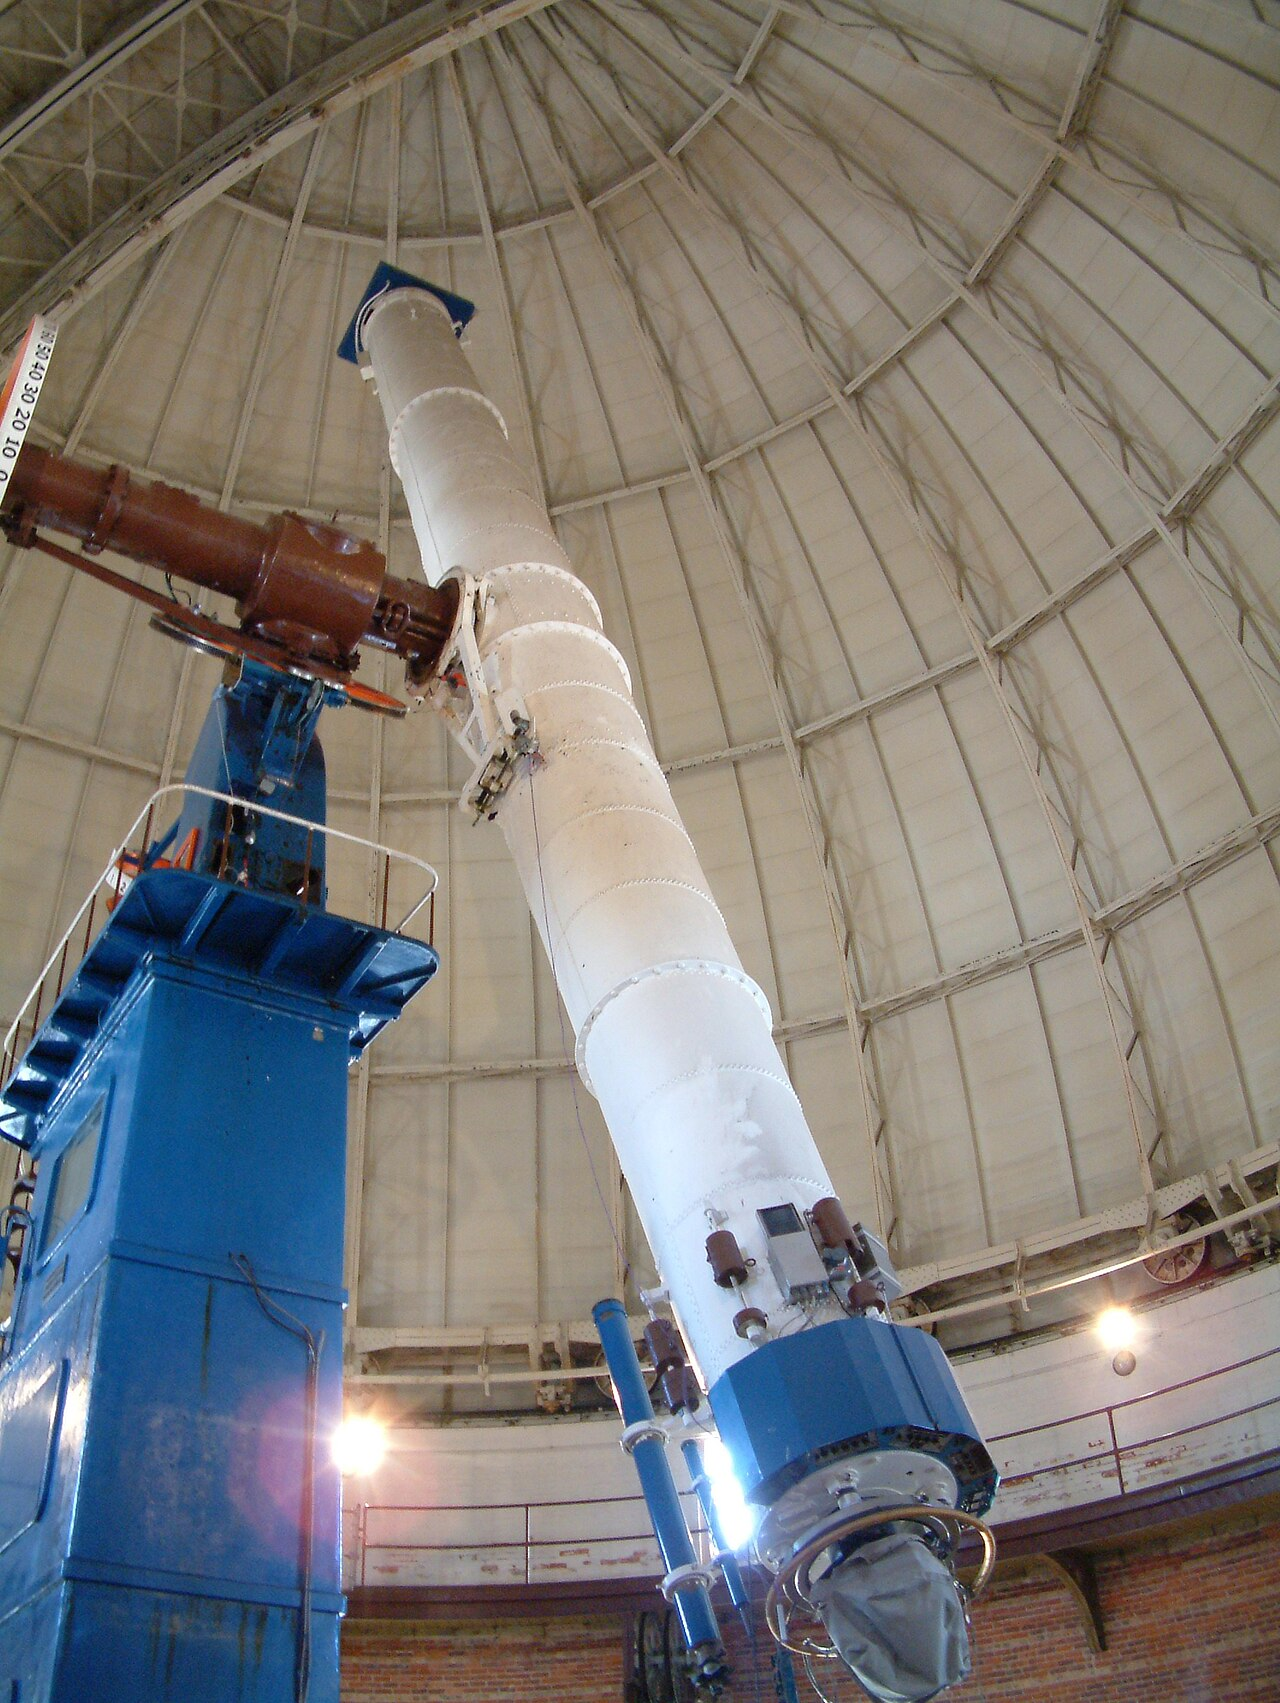
\includegraphics[width=0.42\linewidth]{images/book3/yerkes-refractor.jpg}

{\small Teleskop bias 40 inci Observatorium Yerkes (1897), sampai kini teleskop \omterm{def:b1:mirrors-thin-lenses:lens}{lensa} terbesar yang pernah dibuat: \omterm{def:b1:optical-instruments:microscope}{lensa objektif} sepanjang satu meter dan tabung sepanjang sembilan belas meter. Di atas ukuran ini sebuah \omterm{def:b1:mirrors-thin-lenses:lens}{lensa} melendut oleh beratnya sendiri, dan astronomi pun beralih ke cermin.}
\end{omfigure}

\begin{omfigure}
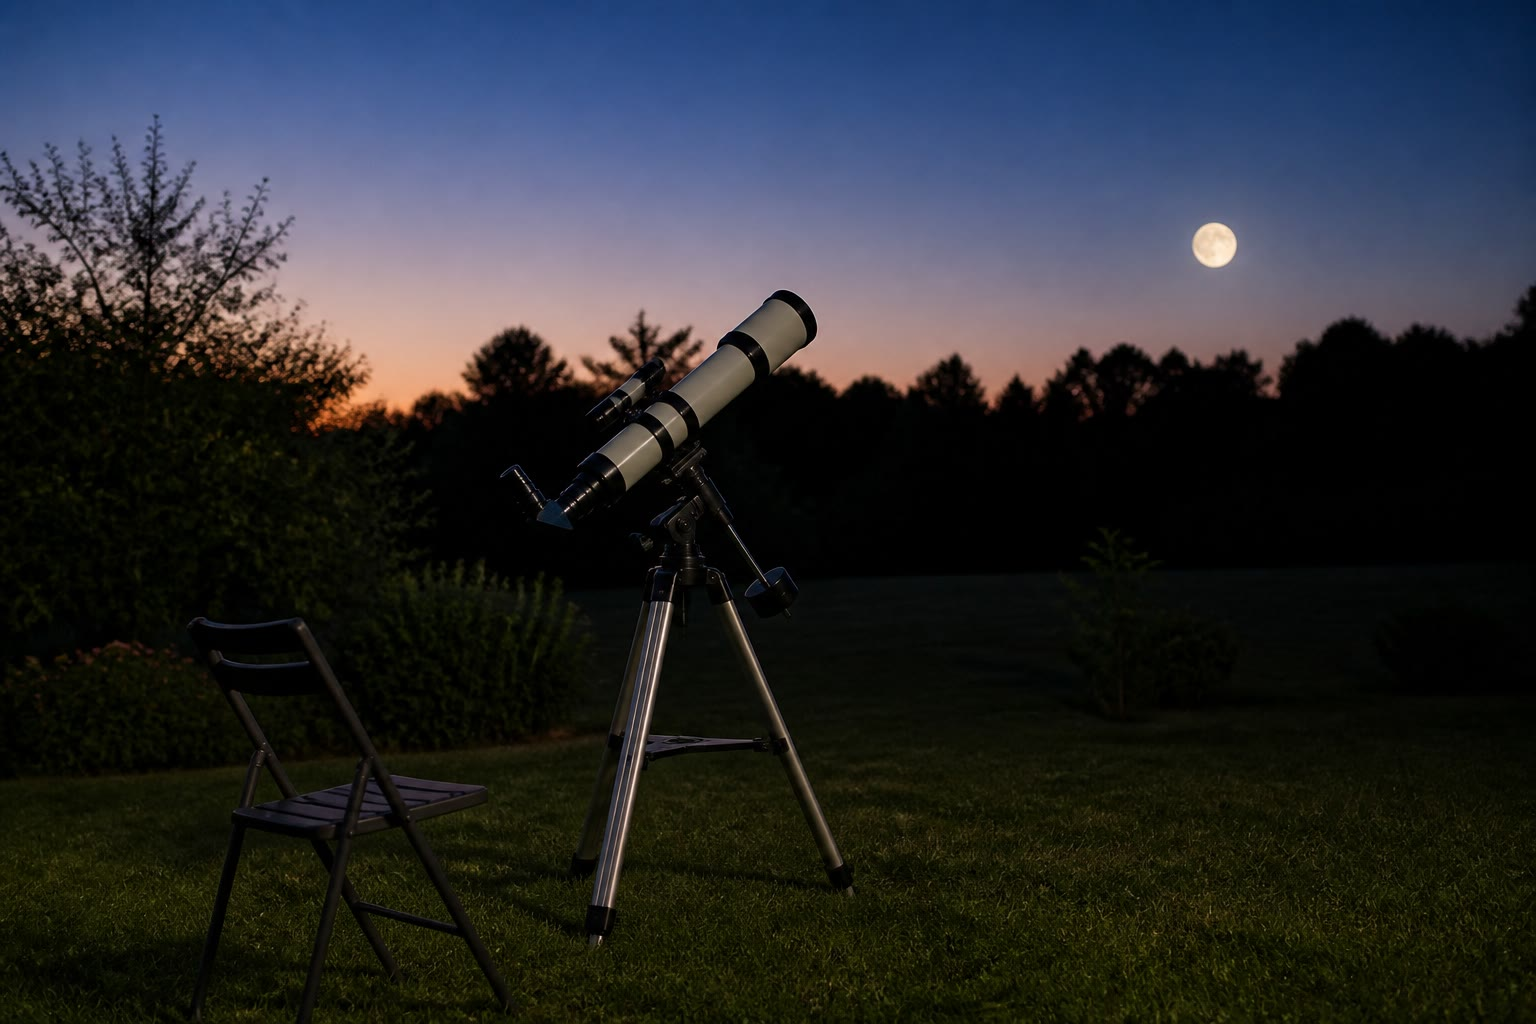
\includegraphics[width=0.58\linewidth]{images/book3/ai/b3-04-telescope-dusk.jpg}

{\small Sebuah teleskop bias kecil pada senja hari: \omterm{def:b1:optical-instruments:microscope}{lensa objektif} berjarak fokus panjang dan \omterm{def:b1:optical-instruments:microscope}{lensa okuler} berjarak fokus pendek --- teleskop afokal bab ini, dibidikkan ke Bulan yang menjadi soal akhir pekannya.}
\end{omfigure}

\section{Mata}

\begin{definition}[Mata tereduksi]\label{def:b1:optical-instruments:eye}
\index{mata}\index{mata tereduksi}\index{retina}\index{akomodasi}
\emph{Mata tereduksi} memodelkan kornea dan \omterm{def:b1:mirrors-thin-lenses:lens}{lensa} matanya sebagai satu
\omterm{def:b1:mirrors-thin-lenses:lens}{lensa tipis} konvergen berjarak fokus \emph{berubah-ubah}, dan
\emph{retina}nya sebagai layar pada jarak tetap $d \approx \qty{17}{mm}$
di belakangnya. Otot mengubah kelengkungan \omterm{def:b1:mirrors-thin-lenses:lens}{lensanya} agar bayangan benda
yang dipandang tetap jatuh di retina: itulah \emph{akomodasi}. Iris di
depan \omterm{def:b1:mirrors-thin-lenses:lens}{lensanya} adalah bukaan berubah-ubah bergaris tengah \qty{2}{}
sampai \qty{8}{mm}, yaitu \emph{pupil}.
\end{definition}

\begin{definition}[Titik jauh, titik dekat]\label{def:b1:optical-instruments:punctum}
\index{titik jauh}\index{titik dekat}\index{amplitudo akomodasi}
\emph{Titik jauh} (punctum remotum) adalah titik benda yang terlihat
tajam tanpa berakomodasi; \emph{titik dekat} (punctum proximum) adalah
titik terdekat yang terlihat tajam dengan \omterm{def:b1:optical-instruments:eye}{akomodasi} maksimum. Bagi \omterm{def:b1:optical-instruments:eye}{mata}
normal (emetrop), titik jauhnya di tak hingga dan titik dekatnya pada
$d_m \approx \qty{25}{cm}$, yaitu \emph{jarak penglihatan jelas} yang
disepakati. Selisih \omterm{def:b1:mirrors-thin-lenses:lens}{vergensi} yang diperlukan untuk keduanya adalah
\emph{amplitudo \omterm{def:b1:optical-instruments:eye}{akomodasi}}: sekitar \qty{4}{\delta} bagi orang dewasa
muda, dan menyusut seiring usia.
\end{definition}

\begin{example}[Vergensi mata]\label{ex:b1:optical-instruments:vergence}
Benda jauh: bayangan pada $d = \qty{17}{mm}$ berarti $f' = \qty{17}{mm}$,
$V = 1/0.017 = \qty{59}{\delta}$. Benda pada \qty{25}{cm}:
$V = 1/0.017 + 1/0.25 = 59 + 4 = \qty{63}{\delta}$. Empat dioptri
\omterm{def:b1:optical-instruments:eye}{akomodasi} dari enam puluh: \omterm{def:b1:mirrors-thin-lenses:lens}{lensa} \omterm{def:b1:optical-instruments:eye}{matanya} hanya menambahkan beberapa
persen pada kerja korneanya, tetapi beberapa persen itulah segalanya
bagi membaca.
\end{example}

\begin{proposition}[Cacat mata dan koreksinya]\label{prop:b1:optical-instruments:defects}
\index{miopi}\index{hipermetropi}\index{presbiopi}
\omterm{def:b1:optical-instruments:eye}{Mata} \emph{miopi} terlalu konvergen: \omterm{def:b1:optical-instruments:punctum}{titik jauhnya} berada pada jarak
berhingga $D_r$; \omterm{def:b1:mirrors-thin-lenses:lens}{lensa divergen} berjarak fokus $f' = -D_r$ (dipakai
dekat \omterm{def:b1:optical-instruments:eye}{mata}) membayangkan tak hingga pada \omterm{def:b1:optical-instruments:punctum}{titik jauhnya} dan memulihkan
penglihatan jauh. \omterm{def:b1:optical-instruments:eye}{Mata} \emph{hipermetropi} kurang konvergen: \omterm{def:b1:optical-instruments:punctum}{titik
jauhnya} maya (di belakang \omterm{def:b1:optical-instruments:eye}{mata}) dan \omterm{def:b1:optical-instruments:punctum}{titik dekatnya} terlalu jauh; \omterm{def:b1:mirrors-thin-lenses:lens}{lensa
konvergen} mengoreksinya. \emph{Presbiopi} adalah hilangnya \omterm{def:b1:optical-instruments:eye}{akomodasi}
seiring usia: \omterm{def:b1:optical-instruments:punctum}{titik dekatnya} mundur dan membaca menuntut \omterm{def:b1:mirrors-thin-lenses:lens}{lensa
konvergen}, apa pun \omterm{def:b1:optical-instruments:punctum}{titik jauhnya}.
\end{proposition}

\begin{proof}
\omterm{def:b1:mirrors-thin-lenses:lens}{Lensa} yang dekat dengan \omterm{def:b1:optical-instruments:eye}{mata} dan \omterm{def:b1:optical-instruments:eye}{mata} itu sendiri membentuk sistem yang
bendanya harus berupa apa yang dapat dilihat \omterm{def:b1:optical-instruments:eye}{matanya}: \omterm{def:b1:mirrors-thin-lenses:lens}{lensanya} harus
mengubah benda di tak hingga menjadi \omterm{def:b1:mirrors-thin-lenses:image}{bayangan maya} di \omterm{def:b1:optical-instruments:punctum}{titik jauhnya},
$\overline{OA'} = -D_r$ untuk $\overline{OA} = -\infty$, sehingga
$f' = \overline{OA'} = -D_r$. Kasus lainnya adalah alasan yang sama
dengan titik-titik yang bersangkutan.
\end{proof}

\begin{omfigure}
\begin{tikzpicture}[font=\small, x=1cm, y=1cm]
  % eye schematic: lens at x=0, retina at x=2.4 (scaled), object far (parallel rays) and near
  \draw[omDef!30, fill=omDef!8] (1.25,0) ellipse (1.45 and 1.15);
  \draw[very thick, omDef, Stealth-Stealth] (0,-0.8) -- (0,0.8);
  \draw[very thick, omThm] (2.6,-0.55) arc (-25:25:1.3);
  \node[omThm, right] at (2.75,0.9) {retina};
  \node[omDef, above] at (0,0.85) {lensa};
  % far object: parallel rays -> focus on retina at axis
  \draw[omProp, -Stealth] (-3.2,0.5) -- (0,0.5); \draw[omProp] (0,0.5) -- (2.58,0);
  \draw[omProp, -Stealth] (-3.2,-0.5) -- (0,-0.5); \draw[omProp] (0,-0.5) -- (2.58,0);
  \draw[-Stealth] (-3.4,0) -- (3.3,0);
  \node[omProp, left] at (-3.2,0.5) {benda jauh};
  \draw[Stealth-Stealth] (0,-1.35) -- (2.58,-1.35) node[midway, below] {$d \approx \qty{17}{mm}$};
  % near object at x=-2.4 height 0.6 : with accommodation image at retina: drawn as converging rays from B through O
  \begin{scope}[xshift=7.6cm]
  \draw[omDef!30, fill=omDef!8] (1.25,0) ellipse (1.45 and 1.15);
  \draw[very thick, omDef, Stealth-Stealth] (0,-0.8) -- (0,0.8);
  \draw[very thick, omThm] (2.6,-0.55) arc (-25:25:1.3);
  \draw[-Stealth] (-3.4,0) -- (3.3,0);
  \draw[very thick, omThm, -Stealth] (-2.6,0) -- (-2.6,0.6); \node[above] at (-2.6,0.6) {$B$};
  \draw[omProp] (-2.6,0.6) -- (0,0.6) -- (2.58,-0.6);
  \draw[omProp] (-2.6,0.6) -- (0,0.0) -- (2.58,-0.6);
  \draw[omProp] (-2.6,0.6) -- (0,-0.6) -- (2.58,-0.6);
  \node[omThm, below right] at (2.55,-0.6) {$B'$};
  \node[below] at (-0.4,-1.3) {berakomodasi: $f'$ memendek};
  \end{scope}
\end{tikzpicture}

{\small \omterm{def:b1:optical-instruments:eye}{Mata tereduksi}: \omterm{def:b1:mirrors-thin-lenses:lens}{lensa tipis} berjarak fokus berubah-ubah dan
\omterm{def:b1:optical-instruments:eye}{retina} \qty{17}{mm} di belakangnya. Ketika rileks, ia memfokuskan benda
jauh; ketika berakomodasi, ia memendekkan $f'$ untuk membawa bayangan
benda dekat ke \omterm{def:b1:optical-instruments:eye}{retinanya}. Bayangannya terbalik --- otaklah yang
membalikkannya kembali.}
\end{omfigure}

\begin{definition}[Ukuran sudut dan daya urai]\label{def:b1:optical-instruments:angular}
\index{ukuran sudut}\index{daya urai sudut}
\emph{Ukuran sudut} sebuah benda setinggi $h$ pada jarak $D$ adalah
$\theta \approx h/D$ (sudut kecil). \omterm{def:b1:optical-instruments:eye}{Mata} membedakan dua titik hanya
jika pisah sudutnya melampaui \emph{\omterm{rem:b1:optical-instruments:abbe}{daya urai} sudut}nya, yaitu sekitar
$\epsilon \approx \qty{3e-4}{rad}$ (satu menit busur): jarak antarsel
kerucutnya dan difraksi pada pupilnya sama-sama menetapkan batas ini.
\end{definition}

\begin{remark}[Untuk apa sebuah alat optik]\label{rem:b1:optical-instruments:purpose}
Dibawa ke \omterm{def:b1:optical-instruments:punctum}{titik dekat}, rincian sebesar \qty{1}{mm} membentang $1/250 =
\qty{4e-3}{rad}$: tiga belas kali batas \omterm{rem:b1:optical-instruments:abbe}{daya urainya}; rincian
\qty{0.05}{mm} membentang $\qty{2e-4}{rad}$ dan tak terlihat. Alat yang
memandang benda dekat (\omterm{def:b1:optical-instruments:G}{kaca pembesar}, \omterm{def:b1:optical-instruments:microscope}{mikroskop}) memperbesar \omterm{def:b1:optical-instruments:angular}{ukuran
sudutnya} melampaui apa yang dapat dicapai dengan mendekatkan bendanya;
alat untuk benda jauh (teleskop) memperbesar \omterm{def:b1:optical-instruments:angular}{ukuran sudut} benda yang
tak dapat didekati; sedangkan \omterm{def:b1:optical-instruments:camera}{kamera} menggantikan \omterm{def:b1:optical-instruments:eye}{retina} dengan sensor
yang dapat mengumpulkan cahaya selama beberapa sekon lalu diperbesar
sesudahnya.
\end{remark}

\section{Kaca pembesar}

\begin{definition}[Perbesaran sudut]\label{def:b1:optical-instruments:G}
\index{perbesaran sudut}\index{kaca pembesar}\index{perbesaran niaga}
Untuk alat yang dipakai \omterm{def:b1:optical-instruments:eye}{mata}, \emph{perbesaran sudut}nya adalah
$G = \theta'/\theta$, dengan $\theta'$ \omterm{def:b1:optical-instruments:angular}{ukuran sudut} bayangan yang
dilihat lewat alatnya dan $\theta$ \omterm{def:b1:optical-instruments:angular}{ukuran sudut} bendanya yang dilihat
\omterm{def:b1:optical-instruments:eye}{mata} telanjang --- pada \omterm{def:b1:optical-instruments:punctum}{titik dekat} $d_m = \qty{25}{cm}$ untuk benda
dekat, dan di tempatnya untuk benda jauh.
\end{definition}

\begin{proposition}[Kaca pembesar]\label{prop:b1:optical-instruments:loupe}
\omterm{def:b1:mirrors-thin-lenses:lens}{Lensa konvergen} berjarak fokus $f' < d_m$ dengan bendanya di bidang
fokus bendanya memberi bayangan di tak hingga, yang terlihat tanpa
\omterm{def:b1:optical-instruments:eye}{akomodasi}, dengan
\[
G = \frac{d_m}{f'} = d_m V .
\]
\end{proposition}

\begin{proof}
Benda $AB$ setinggi $h$ di bidang fokusnya: sinar dari $B$ keluar
sejajar, dengan sudut sinar yang melalui $O$, $\theta' = h/f'$. \omterm{def:b1:optical-instruments:eye}{Mata}
telanjang sebaik-baiknya: $\theta = h/d_m$. Nisbahnya $d_m/f'$.
\end{proof}

\begin{example}[Kaca pembesar tukang jam]\label{ex:b1:optical-instruments:loupe}
$f' = \qty{25}{mm}$: $G = 250/25 = 10$, dijual sebagai ``$10\times$''.
Rincian \qty{0.05}{mm} lalu membentang $\qty{2e-3}{rad}$, terurai dengan
nyaman. Mendorong $G$ lebih tinggi berarti $f'$ beberapa milimeter, yaitu
\omterm{def:b1:mirrors-thin-lenses:lens}{lensa} mungil yang ditempelkan ke \omterm{def:b1:optical-instruments:eye}{mata} --- batas \omterm{def:b1:mirrors-thin-lenses:lens}{lensa} tunggal, dan
alasan keberadaan \omterm{def:b1:optical-instruments:microscope}{mikroskop}.
\end{example}

\section{Mikroskop}

\begin{definition}[Mikroskop majemuk]\label{def:b1:optical-instruments:microscope}
\index{mikroskop}\index{lensa objektif}\index{lensa okuler}\index{selang optik}
\emph{Mikroskop} adalah \emph{\omterm{def:b1:mirrors-thin-lenses:lens}{lensa} objektif} $L_1$ berjarak fokus
pendek $f_1'$ yang membentuk bayangan antara yang nyata dan diperbesar
dari benda yang dekat, tepat di bidang fokus benda sebuah \emph{\omterm{def:b1:mirrors-thin-lenses:lens}{lensa}
okuler} $L_2$ (berjarak fokus $f_2'$), yang berlaku sebagai \omterm{def:b1:optical-instruments:G}{kaca
pembesar}. Jarak $\Delta =
\overline{F_1'F_2}$ antara fokus bayangan
objektifnya dan fokus benda okulernya disebut \emph{selang
optik},
yang dibakukan \qty{160}{mm} pada alat klasik.
\end{definition}

\begin{proposition}[Perbesaran sebuah mikroskop]\label{prop:b1:optical-instruments:microscope}
Dengan bayangan akhirnya di tak hingga,
\[
\gamma_1 = -\frac{\Delta}{f_1'}, \qquad G_2 = \frac{d_m}{f_2'},
\qquad G = \abs{\gamma_1}\,G_2 = \frac{\Delta\,d_m}{f_1' f_2'} .
\]
\end{proposition}

\begin{proof}
Bayangan antaranya $A_1B_1$ terletak di bidang fokus benda \omterm{def:b1:optical-instruments:microscope}{okulernya},
yaitu pada $\overline{F_1'A_1} = \Delta$; \omterm{thm:b1:mirrors-thin-lenses:lensconj}{hubungan Newton} memberi
$\gamma_1 = -\overline{F_1'A_1}/f_1' = -\Delta/f_1'$. \omterm{def:b1:optical-instruments:microscope}{Okulernya} lalu
memperlihatkan $A_1B_1$ (setinggi $\abs{\gamma_1} h$) di tak hingga
dengan sudut $\theta' = \abs{\gamma_1} h/f_2'$, terhadap
$\theta = h/d_m$ bagi \omterm{def:b1:optical-instruments:eye}{mata} telanjang.
\end{proof}

\begin{omfigure}
\begin{tikzpicture}[font=\small, x=1cm, y=1cm]
  % objective L1 at 0, f1'=0.8 ; object at OA=-1.12 -> OA'=2.8, gamma=-2.5 ; eyepiece L2 at 3.8 (f2'=1), F2 = 2.8
  \draw[-Stealth] (-1.9,0) -- (6.7,0);
  \draw[very thick, omDef, Stealth-Stealth] (0,-1.3) -- (0,1.3); \node[omDef, above] at (0,1.35) {objektif $L_1$};
  \draw[very thick, omDef, Stealth-Stealth] (3.8,-1.7) -- (3.8,1.7); \node[omDef, above] at (3.8,1.75) {okuler $L_2$};
  \foreach \x/\n in {-0.8/F_1, 0.8/F_1', 4.8/F_2'} {\fill (\x,0) circle (1.2pt); \node[below] at (\x,-0.05) {$\n$};}
  \fill (2.8,0) circle (1.2pt); \node[above right] at (2.8,0.02) {$F_2$};
  \draw[very thick, omThm, -Stealth] (-1.12,0) -- (-1.12,0.3); \node[above left] at (-1.12,0.3) {$B$};
  \draw[very thick, omThm, -Stealth] (2.8,0) -- (2.8,-0.75); \node[below left] at (2.8,-0.75) {$B_1$};
  \draw[omProp] (-1.12,0.3) -- (0,0.3) -- (2.8,-0.75);
  \draw[omProp] (-1.12,0.3) -- (0,0) -- (2.8,-0.75);
  \draw[omExo] (2.8,-0.75) -- (3.8,-0.75) -- (6.2,1.05);
  \draw[omExo] (2.8,-0.75) -- (3.8,0) -- (6.2,1.8);
  \draw[omExo] (2.8,-0.75) -- (3.8,-1.5) -- (6.2,0.3);
  \draw[Stealth-Stealth] (0.8,0.5) -- (2.8,0.5) node[midway, above] {$\Delta$};
  \node[omExo, right] at (6.25,0.75) {ke mata};
\end{tikzpicture}

{\small \omterm{def:b1:optical-instruments:microscope}{Mikroskop}: \omterm{def:b1:optical-instruments:microscope}{objektifnya} membentuk bayangan antara yang nyata,
diperbesar dan terbalik $A_1B_1$ di bidang fokus benda \omterm{def:b1:optical-instruments:microscope}{okulernya};
\omterm{def:b1:optical-instruments:microscope}{okulernya} mengirimkannya ke tak hingga, tempat \omterm{def:b1:optical-instruments:eye}{mata} yang rileks
memandangnya dengan sudut yang besar.}
\end{omfigure}

\begin{example}[Mikroskop mahasiswa]\label{ex:b1:optical-instruments:micronum}
\omterm{def:b1:optical-instruments:microscope}{Objektif} $f_1' = \qty{4.0}{mm}$, \omterm{def:b1:optical-instruments:microscope}{okuler} $f_2' = \qty{25}{mm}$,
$\Delta = \qty{160}{mm}$: $\gamma_1 = -40$, $G_2 = 10$, $G = 400$.
Bendanya duduk pada $\overline{F_1A} = -f_1'^2/\Delta = -16/160 =
\qty{-0.10}{mm}$ dari $F_1$: \qty{4.1}{mm} dari \omterm{def:b1:optical-instruments:microscope}{objektifnya}. Memfokuskan
berarti menggeser seluruh tabungnya sepersekian milimeter.
\end{example}

\begin{remark}[Batas daya urai]\label{rem:b1:optical-instruments:abbe}
\index{daya urai}
Perbesaran tanpa batas tak akan berguna: cahaya adalah gelombang, dan
\omterm{def:b1:optical-instruments:microscope}{objektif} yang menerima sinar dalam setengah sudut $u$ (di dalam medium
berindeks $n$) tak dapat memisahkan dua titik yang lebih dekat daripada
kira-kira $\lambda/(2n\sin u)$ --- pembahasan gelombang volume Tahun
ke-2 menurunkannya. Dengan $n\sin u \approx 1.4$ (imersi minyak) dan $\lambda =
\qty{0.5}{\micro m}$, batasnya di dekat \qty{0.2}{\micro m}. Agar
rincian itu terlihat \omterm{def:b1:optical-instruments:eye}{mata} ($\epsilon = \qty{3e-4}{rad}$ pada
\qty{25}{cm}, yaitu \qty{75}{\micro m}), perbesaran sekitar $400$ sudah
cukup; di atas $1000$ bayangannya hanya lebih besar, bukan lebih kaya:
\emph{perbesaran hampa}.
\end{remark}

\section{Teleskop astronomi}

\begin{proposition}[Teleskop bias]\label{prop:b1:optical-instruments:telescope}
\index{teleskop}\index{pupil keluar}
\omterm{def:b1:optical-instruments:microscope}{Lensa objektif} $L_1$ dan \omterm{def:b1:optical-instruments:microscope}{lensa okuler} $L_2$ dengan $F_1' = F_2$
membentuk \omterm{prop:b1:mirrors-thin-lenses:doublet}{sistem afokal}: sebuah bintang (di tak hingga) terlihat di tak
hingga, \omterm{def:b1:optical-instruments:eye}{mata} yang rileks memandangnya, dan
\[
G = -\frac{f_1'}{f_2'} .
\]
Bayangan tepi \omterm{def:b1:optical-instruments:microscope}{objektifnya} lewat \omterm{def:b1:optical-instruments:microscope}{okulernya} disebut \emph{\omterm{prop:b1:optical-instruments:telescope}{pupil keluar}}:
cakram terang bergaris tengah $D/\abs G$ yang terletak
$\overline{O_2P'} = f_2'(f_1' + f_2')/f_1'$ di belakang \omterm{def:b1:optical-instruments:microscope}{okulernya},
tempat pupil \omterm{def:b1:optical-instruments:eye}{mata} harus diletakkan agar menerima seluruh cahayanya.
\end{proposition}

\begin{proof}
$G$ telah diturunkan dalam \cref{prop:b1:mirrors-thin-lenses:doublet}.
\omterm{def:b1:optical-instruments:microscope}{Objektifnya}, dilihat dari $L_2$, adalah benda pada $\overline{O_2O_1} = -(f_1'
+ f_2')$; Descartes memberi $1/\overline{O_2P'} = 1/f_2' - 1/(f_1' + f_2')
= f_1'/[f_2'(f_1' + f_2')]$, dan perbesarannya $\overline{O_2P'}/
\overline{O_2O_1} = -f_2'/f_1' = 1/G$ menskalakan garis tengah $D$
menjadi $D/\abs G$. Setiap sinar yang masuk ke \omterm{def:b1:optical-instruments:microscope}{objektifnya} keluar lewat
\omterm{prop:b1:optical-instruments:telescope}{pupil keluarnya}, karena setiap titik \omterm{def:b1:optical-instruments:microscope}{objektifnya} dibayangkan di sana.
\end{proof}

\begin{omfigure}
\begin{tikzpicture}[font=\small, x=1cm, y=1cm]
  % objective f1'=4 at x=0 ; eyepiece f2'=1 at x=5 ; parallel beam at angle alpha -> focus at height -4*alpha; take alpha such that height 0.5: rays entering at heights 1, 0, -1 with slope -0.125
  \draw[-Stealth] (-2.2,0) -- (7.8,0);
  \draw[very thick, omDef, Stealth-Stealth] (0,-1.4) -- (0,1.4); \node[omDef, above] at (0,1.45) {objektif $L_1$, $D$};
  \draw[very thick, omDef, Stealth-Stealth] (5,-0.8) -- (5,0.8); \node[omDef, above] at (5,0.85) {okuler $L_2$};
  \fill (4,0) circle (1.2pt); \node[above] at (4,0.08) {$F_1' = F_2$};
  % beam from a star at angle: parallel rays slope -0.125 entering at y=1.25,0.25,-0.75 then reaching lens; then to focus (4,-0.5)
  \foreach \y in {1.2,0.0,-1.2} {
    \draw[omProp] (-2.0,\y+0.25) -- (0,\y);
    \draw[omProp] (0,\y) -- (4,-0.5);
    % after eyepiece: parallel, slope = +0.5/1 -> direction from (5, y2) with slope 0.5; y2 = -0.5 + (4,-0.5)->(5,?) line through focus continuing: ray from (0,\y) to (4,-0.5) extended to x=5: y = -0.5 + (-0.5-\y)/4
    \draw[omExo] (4,-0.5) -- (5,{-0.5+(-0.5-\y)/4}) -- (7.6,{-0.5+(-0.5-\y)/4+1.3});
  }
  % exit pupil: image of objective rim: O2P' = 1*5/4 = 1.25 beyond L2 ; diameter D/G = 2.4/4 = 0.6
  \draw[very thick, omThm] (6.25,-0.3) -- (6.25,0.3); \node[omThm, below] at (6.4,-0.8) {pupil keluar $D/\abs{G}$};
  \node[omProp, left] at (-2.0,1.45) {dari sebuah bintang};
\end{tikzpicture}

{\small Teleskop astronomi: berkas sejajar dari sebuah bintang
difokuskan \omterm{def:b1:optical-instruments:microscope}{objektifnya} di bidang fokus bersamanya lalu dikirim kembali
ke tak hingga oleh \omterm{def:b1:optical-instruments:microscope}{okulernya}, dengan sudut $\abs G$ kali lebih besar.
Seluruh cahaya yang dikumpulkan \omterm{def:b1:optical-instruments:microscope}{objektif} bergaris tengah $D$ melewati
\omterm{prop:b1:optical-instruments:telescope}{pupil keluarnya}, yang bergaris tengah $D/\abs G$.}
\end{omfigure}

\begin{proposition}[Apa yang diperoleh sebuah teleskop]\label{prop:b1:optical-instruments:gains}
\index{daya kumpul cahaya}\index{kriteria Rayleigh}
Dibandingkan dengan \omterm{def:b1:optical-instruments:eye}{mata} telanjang (pupil $d_p$):
\begin{itemize}
  \item \emph{\omterm{def:b1:optical-instruments:angular}{ukuran sudut}}: dikalikan $\abs G$;
  \item \emph{cahaya yang terkumpul} dari sumber titik: dikalikan
        $(D/d_p)^2$, asalkan \omterm{prop:b1:optical-instruments:telescope}{pupil keluarnya} tidak lebih besar daripada
        pupil \omterm{def:b1:optical-instruments:eye}{matanya}, yaitu $\abs G \geq D/d_p$;
  \item \emph{\omterm{def:b1:optical-instruments:angular}{daya urai sudut}}: difraksi pada \omterm{def:b1:optical-instruments:microscope}{objektifnya} membatasinya
        pada $\theta_{\min} \approx 1.22\,\lambda/D$ (kriteria
        Rayleigh), jauh di bawah $\epsilon$ milik \omterm{def:b1:optical-instruments:eye}{mata}; perbesaran yang
        membuat batas ini terlihat adalah $G_r = \epsilon/\theta_{\min}$,
        dan perbesaran yang lebih besar hanya memperbesar kekaburannya.
\end{itemize}
\end{proposition}
\admitted

\begin{example}[Teleskop bias 150 milimeter seorang amatir]\label{ex:b1:optical-instruments:telnum}
$D = \qty{150}{mm}$, $f_1' = \qty{1200}{mm}$, \omterm{def:b1:optical-instruments:microscope}{okuler} \qty{25}{mm}:
$G = -48$; \omterm{prop:b1:optical-instruments:telescope}{pupil keluarnya} \qty{3.1}{mm}; penguatan cahayanya $(150/7)^2 \approx
460$ terhadap pupil yang teradaptasi gelap sebesar \qty{7}{mm}; \omterm{rem:b1:optical-instruments:abbe}{daya
urainya} $1.22 \times
\qty{550}{nm}/\qty{0.15}{m} = \qty{4.5e-6}{rad} = 0.9''$, sehingga kawah
selebar \qty{1.7}{km} di Bulan; $G_r = 3\times10^{-4}/4.5\times
10^{-6} \approx 67$ --- \omterm{def:b1:optical-instruments:microscope}{okuler} \qty{6}{mm} ($G = 200$) tak
memperlihatkan rincian lebih banyak, hanya cakram yang lebih besar dan
lebih pudar. Soal akhir pekan merancang alat ini.
\end{example}

\begin{remark}[Teleskop pantul, teropong binokuler, teropong Galileo]\label{rem:b1:optical-instruments:variants}
\omterm{def:b1:mirrors-thin-lenses:mirror}{Cermin cekung} berjarak fokus $f_1'$ menggantikan \omterm{def:b1:optical-instruments:microscope}{lensa objektif} dalam
teleskop \emph{pantul} (tanpa dispersi warna, dan cermin dapat dibuat
selebar beberapa meter serta ditopang dari belakang): segala hal di atas
tetap berlaku dengan $f_1'$ sebagai \omterm{def:b1:mirrors-thin-lenses:lens}{jarak fokus} cerminnya. Bayangannya
terbalik --- tak berbahaya bagi bintang; untuk pemakaian di bumi,
teropong binokuler menyisipkan sepasang prisma pemantul sempurna untuk
menegakkannya, dan teropong Galileo memakai \omterm{def:b1:optical-instruments:microscope}{okuler} divergen
($f_2' < 0$, $G > 0$), lebih pendek tetapi bermedan pandang sempit.
\end{remark}

\section{Kamera}

\begin{definition}[Kamera; bilangan-f]\label{def:b1:optical-instruments:camera}
\index{kamera}\index{bilangan-f}\index{kedalaman medan}
\emph{Kamera} adalah \omterm{def:b1:mirrors-thin-lenses:lens}{lensa konvergen} berjarak fokus $f'$ yang membentuk
\omterm{def:b1:mirrors-thin-lenses:image}{bayangan nyata} pada sensor, pada $\overline{OA'} \approx f'$ untuk objek
jauh; memfokuskannya berarti menggeser \omterm{def:b1:mirrors-thin-lenses:lens}{lensanya}. Diafragma bergaris
tengah $D$ membatasi berkasnya; \emph{bilangan-f}nya adalah
$N = f'/D$ (ditulis $f/N$). \emph{Sudut pandang}nya adalah
$2\arctan(\ell/2f')$ untuk sensor selebar $\ell$.
\end{definition}

\begin{proposition}[Pajanan dan kedalaman medan]\label{prop:b1:optical-instruments:dof}
\index{jarak hiperfokal}
Iradiansi pada sensornya menskala sebagai $1/N^2$, sehingga waktu
pajanan untuk kecerahan bayangan tertentu menskala sebagai $N^2$. Titik
yang berjarak lain daripada jarak yang difokuskan membentuk cakram
kabur; dengan menuntut cakram itu tetap di bawah garis tengah yang
ditoleransi $c$, \omterm{def:b1:mirrors-thin-lenses:lens}{lensa} yang difokuskan pada \emph{\omterm{prop:b1:optical-instruments:dof}{jarak hiperfokal}}
\[
H = \frac{f'^2}{N c}
\]
membuat segala sesuatu dari $H/2$ sampai tak hingga tampak cukup tajam.
\end{proposition}

\begin{proof}
Iradiansi $=$ daya/luas $\propto D^2/f'^2 = 1/N^2$ (bayangan objek
tertentu berukuran tetap yang ditetapkan $f'$, sedangkan daya yang
terkumpul tumbuh sebagai $D^2$). Fokuskan pada jarak $p$ dengan
bayangannya di $q \approx f'$; titik di tak hingga memfokus di $f'$,
yaitu $q - f'$ sebelum sensornya; kerucut sinarnya, yang beralas $D$ di
\omterm{def:b1:mirrors-thin-lenses:lens}{lensanya}, bergaris tengah $D(q - f')/q$ pada sensornya (segitiga
sebangun). Dengan $1/q = 1/f' - 1/p$ secara paraksial,
$q - f' \approx f'^2/p$ untuk $p \gg f'$, sehingga kekaburannya
$Df'/p = f'^2/(Np)$; ia sama dengan $c$ ketika $p = H$. Geometri yang
sama pada sisi dekatnya memberi batas $H/2$.
\end{proof}

\begin{omfigure}
\begin{tikzpicture}[font=\small, x=1cm, y=1cm]
  \draw[-Stealth] (-5.5,0) -- (2.6,0);
  \draw[very thick, omDef, Stealth-Stealth] (0,-1.2) -- (0,1.2); \node[omDef, above] at (0,1.25) {lensa, bukaan $D$};
  \draw[very thick] (1.8,-1.3) -- (1.8,1.3); \node[right] at (1.8,1.1) {sensor};
  % focused point at x=-4 (p) images at q=1.8 ; far point at infinity images at f'=1.5
  \fill[omThm] (-4,0) circle (1.5pt); \node[below left, omThm] at (-4,-0.05) {titik yang difokuskan};
  \draw[omThm] (-4,0) -- (0,1.0) -- (1.8,0); \draw[omThm] (-4,0) -- (0,-1.0) -- (1.8,0);
  % far point: parallel rays focus at 1.5, then diverge to sensor making blur
  \draw[omProp] (-5.3,1.0) -- (0,1.0) -- (1.5,0) -- (1.8,-0.2);
  \draw[omProp] (-5.3,-1.0) -- (0,-1.0) -- (1.5,0) -- (1.8,0.2);
  \draw[very thick, omProp] (1.82,-0.2) -- (1.82,0.2); \node[omProp, right] at (1.85,-0.35) {kabur $c$};
  \node[omProp, left] at (-5.3,1.0) {titik jauh};
  \fill (1.5,0) circle (1.2pt); \node[below] at (1.5,-0.05) {$F'$};
\end{tikzpicture}

{\small \omterm{def:b1:optical-instruments:camera}{Kedalaman medan}: \omterm{def:b1:mirrors-thin-lenses:lens}{lensanya} difokuskan pada titik berjarak $p$
(bayangannya di sensor); titik di tak hingga memfokus di $F'$, sebelum
sensornya, dan meninggalkan cakram kabur bergaris tengah $c = Df'/p$ ---
lebih kecil untuk bukaan kecil ($N$ besar), karena itu ada tukar-tambah
antara ketajaman dan waktu pajanan.}
\end{omfigure}

\begin{example}[Bingkai penuh dan telepon]\label{ex:b1:optical-instruments:cameras}
\omterm{def:b1:mirrors-thin-lenses:lens}{Lensa} \qty{50}{mm} pada sensor selebar \qty{36}{mm}: sudut pandangnya
$2\arctan(18/50) = 40^\circ$; pada $f/8$ dengan $c = \qty{0.03}{mm}$,
$H = 2500/(8 \times 0.03) = \qty{10}{m}$: difokuskan pada \qty{10}{m},
segala sesuatu di luar \qty{5}{m} menjadi tajam. \omterm{def:b1:mirrors-thin-lenses:lens}{Lensa} telepon,
$f' = \qty{4.3}{mm}$ pada $f/1.8$ dengan sensor \qty{6}{mm} dan
$c = \qty{5}{\micro m}$: sudut pandang yang sama
(selebar \qty{70}{\degree}), $H = 18.5/(1.8 \times 0.005) =
\qty{2.1}{m}$ --- hampir segala sesuatu terfokus sekaligus, itulah
sebabnya telepon memalsukan kaburnya latar belakang dengan perangkat lunak.
\end{example}

\begin{omfigure}
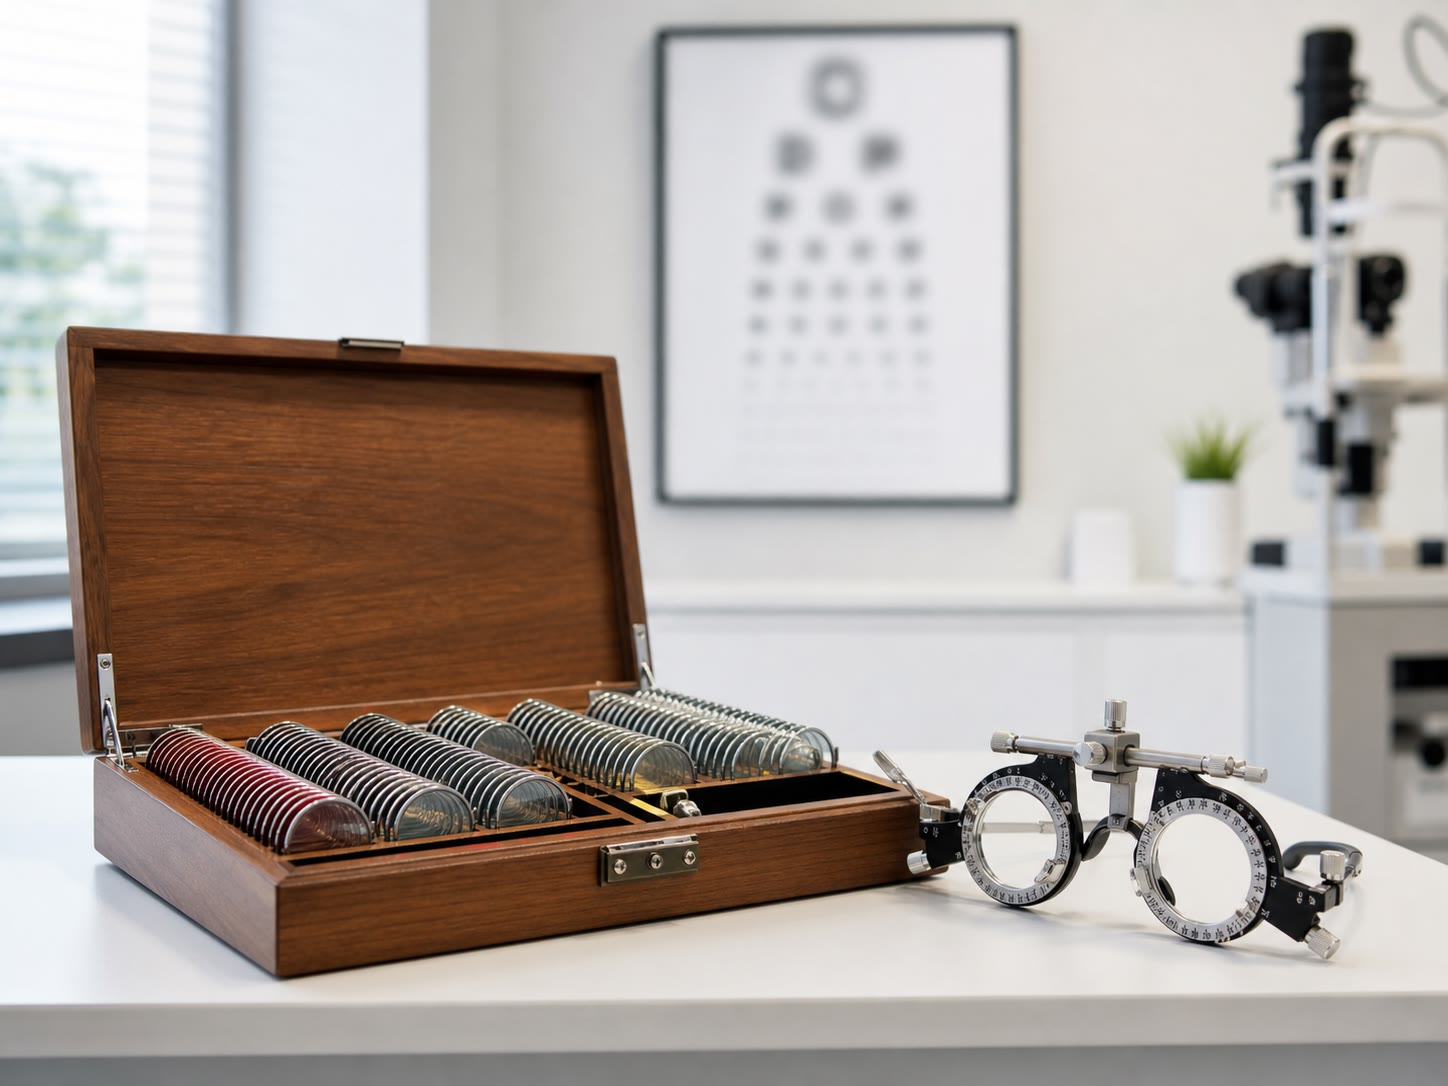
\includegraphics[width=0.50\linewidth]{images/book3/ai/b3-04-eye-chart-trial-frame.jpg}

{\small \omterm{def:b1:mirrors-thin-lenses:lens}{Lensa} uji dan bingkai uji milik optometris: \omterm{def:b1:mirrors-thin-lenses:lens}{lensa konvergen} atau divergen dengan \omterm{def:b1:mirrors-thin-lenses:lens}{vergensi} yang tepat di depan \omterm{def:b1:optical-instruments:eye}{mata} memindahkan \omterm{def:b1:optical-instruments:punctum}{titik jauhnya} kembali ke tak hingga.}
\end{omfigure}

\section{Latihan}

\begin{exercise}[$\star$]\label{exo:b1:optical-instruments:1}
Dengan \omterm{def:b1:optical-instruments:eye}{retina} \qty{17}{mm} di belakang \omterm{def:b1:mirrors-thin-lenses:lens}{lensanya}, hitunglah \omterm{def:b1:mirrors-thin-lenses:lens}{vergensi} \omterm{def:b1:optical-instruments:eye}{mata}
normal yang memandang tak hingga, lalu yang memandang \qty{25}{cm};
simpulkan \omterm{def:b1:optical-instruments:punctum}{amplitudo akomodasinya}. Berapa \omterm{def:b1:mirrors-thin-lenses:lens}{jarak fokus} keduanya?
\end{exercise}

\begin{exercise}[$\star$]\label{exo:b1:optical-instruments:2}
\omterm{def:b1:optical-instruments:eye}{Mata} miopi mempunyai \omterm{def:b1:optical-instruments:punctum}{titik jauh} pada \qty{40}{cm}. \omterm{def:b1:mirrors-thin-lenses:lens}{Lensa} apa yang
mengoreksinya (\omterm{def:b1:mirrors-thin-lenses:lens}{jarak fokus}, \omterm{def:b1:mirrors-thin-lenses:lens}{vergensi})? \omterm{def:b1:optical-instruments:eye}{Mata} hipermetropi tak dapat
berakomodasi pada apa pun yang lebih dekat daripada \qty{1.0}{m}: \omterm{def:b1:mirrors-thin-lenses:lens}{lensa}
apa yang memungkinkannya membaca pada \qty{25}{cm}?
\end{exercise}

\begin{exercise}[$\star$]\label{exo:b1:optical-instruments:3}
\omterm{def:b1:optical-instruments:G}{Kaca pembesar} mempunyai $f' = \qty{4.0}{cm}$. Berikan \omterm{def:b1:optical-instruments:G}{perbesaran
sudutnya}, di mana perangkonya harus dipegang, dan \omterm{def:b1:optical-instruments:angular}{ukuran sudut} rincian
\qty{2}{mm} lewat kaca itu, dibandingkan dengan \omterm{def:b1:optical-instruments:eye}{mata} telanjang pada \qty{25}{cm}.
\end{exercise}

\begin{exercise}[$\star$]\label{exo:b1:optical-instruments:4}
Teleskop bias mempunyai $f_1' = \qty{900}{mm}$. Hitunglah $G$ dengan
\omterm{def:b1:optical-instruments:microscope}{okuler} \qty{25}{mm} dan dengan \omterm{def:b1:optical-instruments:microscope}{okuler} \qty{9}{mm}, panjang tabungnya
pada tiap kasus, dan ukuran semu Bulan ($0.52^\circ$).
\end{exercise}

\begin{exercise}[$\star\star$]\label{exo:b1:optical-instruments:5}
\omterm{def:b1:optical-instruments:microscope}{Mikroskop}: $f_1' = \qty{4.0}{mm}$, $f_2' = \qty{20}{mm}$,
$\Delta = \qty{160}{mm}$. Hitunglah $\gamma_1$, $G_2$, $G$, dan jarak
benda--objektifnya. Sejauh apa tabungnya harus bergeser untuk membawa
bendanya \qty{10}{\micro m} lebih dalam ke dalam fokus?
\end{exercise}

\begin{exercise}[$\star\star$]\label{exo:b1:optical-instruments:6}
Dua lampu depan berjarak \qty{1.5}{m}. Dari jarak berapa \omterm{def:b1:optical-instruments:eye}{mata} telanjang
($\epsilon = \qty{3e-4}{rad}$) dapat membedakan keduanya? Sebuah
teleskop dengan $D = \qty{100}{mm}$: hitunglah batas difraksinya ($\lambda =
\qty{550}{nm}$), jarak yang masih memisahkan kedua lampu itu, dan
perbesaran $G_r$ yang di atasnya ia tak memperlihatkan apa pun yang baru.
\end{exercise}

\begin{exercise}[$\star\star$]\label{exo:b1:optical-instruments:7}
\omterm{def:b1:mirrors-thin-lenses:lens}{Lensa} \qty{50}{mm} pada $f/2$: berapa garis tengah bukaannya? Sebuah
pemandangan terpajan dengan benar pada $f/2$ selama $1/500$~\unit{s};
berapa waktu pajanan pada $f/8$? Apa yang dibeli bukaan yang lebih kecil?
\end{exercise}

\begin{exercise}[$\star\star$]\label{exo:b1:optical-instruments:8}
Hitunglah \omterm{prop:b1:optical-instruments:dof}{jarak hiperfokal} \omterm{def:b1:mirrors-thin-lenses:lens}{lensa} \qty{35}{mm} pada $f/11$ dengan
$c = \qty{0.03}{mm}$, dan rentang jarak yang tajam ketika ia
difokuskan pada $H$. Pemotret jalanan menyetelnya lebih dulu: mengapa?
\end{exercise}

\begin{exercise}[$\star\star$]\label{exo:b1:optical-instruments:9}
Teropong binokuler ``$8\times30$'' mempunyai $G = 8$ dan
$D = \qty{30}{mm}$. Hitunglah \omterm{prop:b1:optical-instruments:telescope}{pupil keluarnya}; apakah seluruh cahayanya
terpakai oleh pupil malam \qty{7}{mm}? Bagaimana untuk ``$7\times50$''?
Pasangan mana yang lebih baik pada senja hari, dan mengapa
``$20\times30$'' merupakan pilihan yang buruk?
\end{exercise}

\begin{exercise}[$\star\star\star$]\label{exo:b1:optical-instruments:10}
\omterm{def:b1:optical-instruments:punctum}{Titik jauh} seorang miopi berada \qty{25}{cm} dari \omterm{def:b1:optical-instruments:eye}{matanya}. Hitunglah
\omterm{def:b1:mirrors-thin-lenses:lens}{vergensi} \omterm{def:b1:mirrors-thin-lenses:lens}{lensa} kontak yang mengoreksinya, lalu \omterm{def:b1:mirrors-thin-lenses:lens}{vergensi} \omterm{def:b1:mirrors-thin-lenses:lens}{lensa} kacamata
yang dipakai \qty{15}{mm} di depan \omterm{def:b1:optical-instruments:eye}{matanya}. Koreksi mana yang lebih
kuat, dan mengapa keduanya berbeda?
\end{exercise}

\begin{exercise}[$\star\star\star$]\label{exo:b1:optical-instruments:11}
Teropong Galileo: $f_1' = \qty{30}{cm}$, $f_2' = \qty{-10}{cm}$.
Carilah pisah \omterm{def:b1:mirrors-thin-lenses:lens}{lensanya} agar sistemnya afokal, $G$, dan arah bayangannya.
Tentukan letak \omterm{prop:b1:optical-instruments:telescope}{pupil keluarnya} lalu jelaskan mengapa medan pandangnya sempit.
\end{exercise}

\begin{exercise}[$\star\star\star$]\label{exo:b1:optical-instruments:12}
Sebuah teleskop \qty{200}{mm} dan pupil \qty{7}{mm}. Dengan faktor
berapa cahaya dari sebuah bintang bertambah? Astronom menilai kecerahan
dengan magnitudo, $m_2 - m_1 = 2.5\log_{10}(F_1/F_2)$; \omterm{def:b1:optical-instruments:eye}{mata} mencapai
magnitudo $6$: magnitudo pembatas berapa yang diberikan teleskop itu?
Berapa kali lebih jauh sebuah lampu tertentu dapat terlihat?
\end{exercise}

\begin{omfigure}
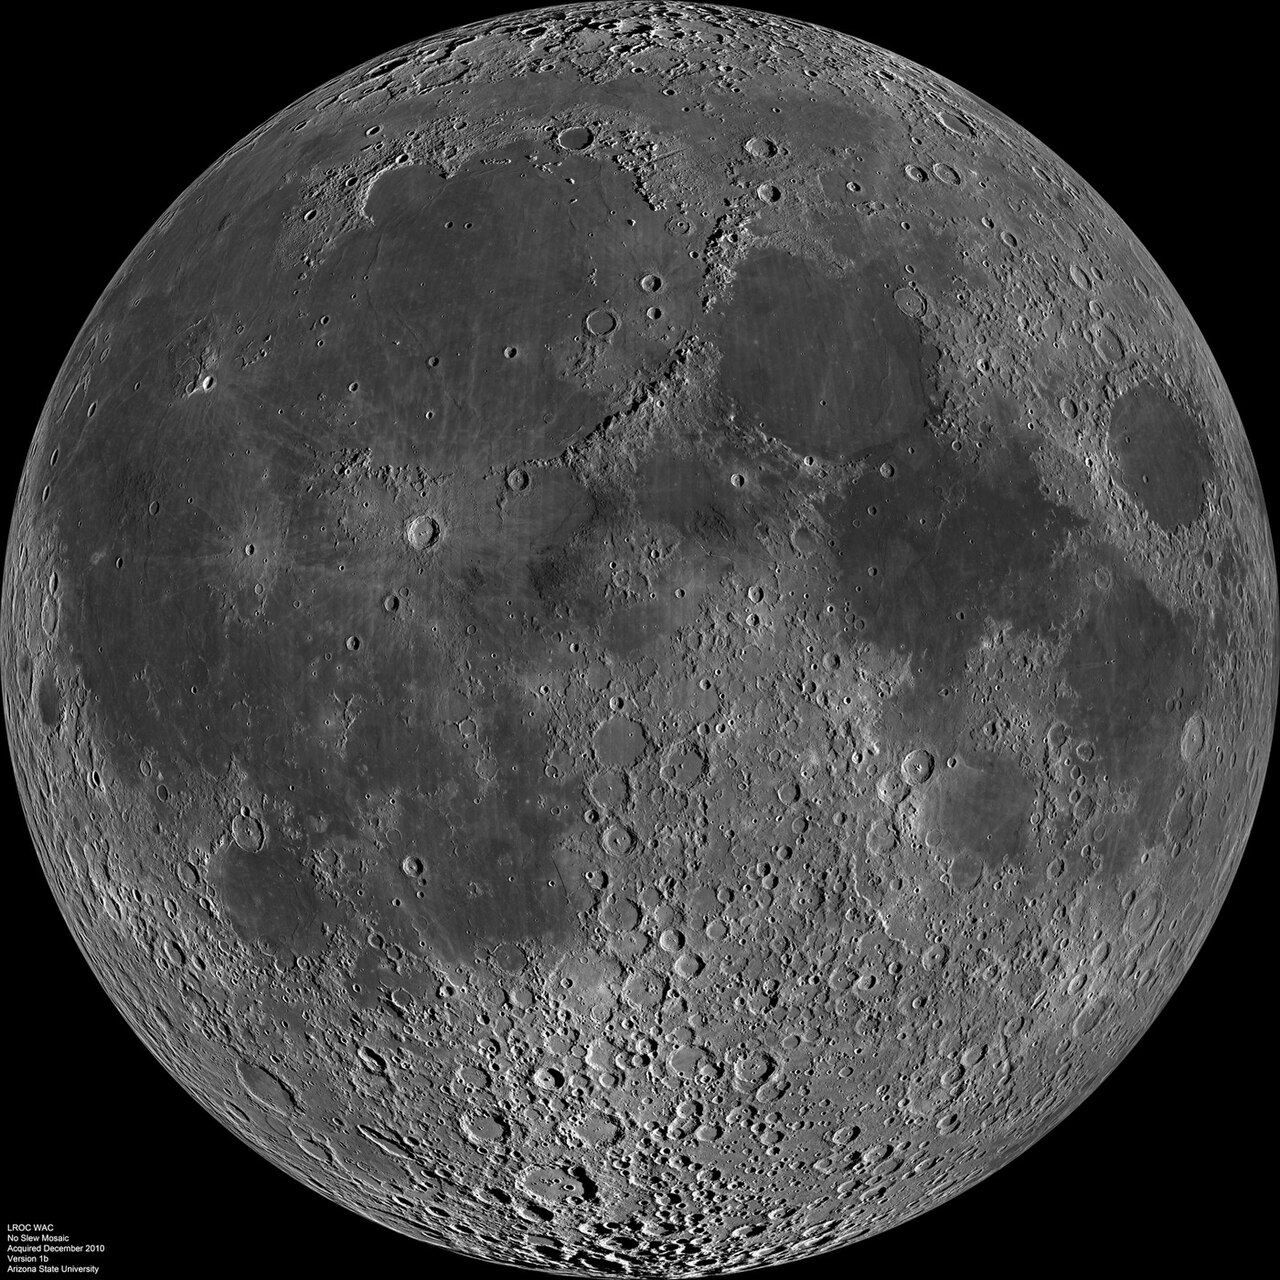
\includegraphics[width=0.40\linewidth]{images/book3/moon-nearside-lro.jpg}

{\small Sisi dekat Bulan (LRO, NASA): sasaran teleskop pada soal akhir pekan, selebar \qty{3476}{km} pada jarak \qty{384000}{km}.}
\end{omfigure}

\section{Soal: Merancang teleskop untuk Bulan}

\begin{problem}[{Soal akhir pekan --- teleskop bias 150 milimeter di
halaman rumput: pilih okulernya, tempatkan matanya, hitung cahayanya,
lalu cari tahu sekecil apa kawah yang dapat diperlihatkannya}]
\label{pb:b1:optical-instruments:1}
\omterm{def:b1:optical-instruments:microscope}{Lensa objektifnya} adalah \omterm{def:b1:mirrors-thin-lenses:lens}{lensa konvergen} $L_1$ berjarak fokus
$f_1' = \qty{1200}{mm}$ dan bergaris tengah $D = \qty{150}{mm}$; tersedia
\omterm{def:b1:optical-instruments:microscope}{okuler} $L_2$ berjarak fokus \qty{25}{mm} dan \qty{6}{mm}. Bulan berjarak
\qty{3.84e5}{km} dan membentang $0.52^\circ$; pupil malam \omterm{def:b1:optical-instruments:eye}{matanya}
\qty{7}{mm}, \omterm{rem:b1:optical-instruments:abbe}{daya urainya} $\epsilon = \qty{3.0e-4}{rad}$;
$\lambda = \qty{550}{nm}$.

\medskip
\noindent\textbf{Bagian I --- Susunan afokal.}
\begin{enumerate}
  \item Di mana \omterm{def:b1:optical-instruments:microscope}{okulernya} harus ditempatkan agar sebuah bintang terlihat
        tanpa \omterm{def:b1:optical-instruments:eye}{akomodasi}? Berikan jarak objektif--okuler untuk tiap
        \omterm{def:b1:optical-instruments:microscope}{okulernya}.
  \item Periksalah dengan \omterm{thm:b1:mirrors-thin-lenses:lensconj}{hubungan Descartes}, yang diterapkan pada tiap
        \omterm{def:b1:mirrors-thin-lenses:lens}{lensa} berturut-turut, bahwa titik di tak hingga pada sumbunya
        dibayangkan di tak hingga.
  \item Tunjukkan bahwa berkas dari bintang bersudut $\alpha$ terhadap
        sumbunya keluar sebagai berkas sejajar bersudut
        $\alpha' = -(f_1'/f_2')\alpha$.
  \item Hitunglah $G$ untuk tiap \omterm{def:b1:optical-instruments:microscope}{okulernya} dan garis tengah semu Bulan
        lewat masing-masingnya.
  \item Bayangannya terbalik. Mengapa hal itu dapat diterima di sini,
        dan apa yang akan ditambahkan sebuah teropong pengamat di bumi?
  \item Di mana bayangan antara Bulan yang nyata itu berada, dan berapa
        garis tengahnya? (Ia dapat difoto di sana.)
\end{enumerate}

\medskip
\noindent\textbf{Bagian II --- Ke mana \omterm{def:b1:optical-instruments:eye}{matanya} diletakkan.}
\begin{enumerate}[resume]
  \item Tunjukkan bahwa \omterm{def:b1:optical-instruments:microscope}{okulernya} membentuk \omterm{def:b1:mirrors-thin-lenses:image}{bayangan nyata} tepi
        \omterm{def:b1:optical-instruments:microscope}{objektifnya} pada $\overline{O_2P'} = f_2'(f_1' + f_2')/f_1'$ di
        belakangnya, bergaris tengah $D/\abs G$ (\omterm{prop:b1:optical-instruments:telescope}{pupil keluarnya}).
  \item Hitunglah kedudukan dan garis tengah \omterm{prop:b1:optical-instruments:telescope}{pupil keluarnya} untuk tiap
        \omterm{def:b1:optical-instruments:microscope}{okulernya}.
  \item Mengapa pupil \omterm{def:b1:optical-instruments:eye}{matanya} harus diletakkan pada \omterm{prop:b1:optical-instruments:telescope}{pupil keluarnya}? Apa
        yang terjadi pada medan pandangnya jika ia diletakkan lebih ke
        belakang?
  \item Agar cahaya sebuah bintang terpakai sepenuhnya, \omterm{prop:b1:optical-instruments:telescope}{pupil keluarnya}
        tak boleh melampaui pupil \omterm{def:b1:optical-instruments:eye}{matanya}: simpulkan perbesaran berguna
        minimum teleskop ini pada malam hari.
\end{enumerate}

\medskip
\noindent\textbf{Bagian III --- \omterm{rem:b1:optical-instruments:abbe}{Daya urai}.}
\begin{enumerate}[resume]
  \item Hitunglah batas difraksinya $\theta_{\min} = 1.22\lambda/D$
        dalam radian dan dalam detik busur.
  \item Kawah sekecil apa yang bersesuaian dengan sudut ini di Bulan?
        Dan bagi \omterm{def:b1:optical-instruments:eye}{mata} telanjang?
  \item Definisikan lalu hitunglah perbesaran pengurai $G_r =
        \epsilon/\theta_{\min}$. \omterm{def:b1:optical-instruments:microscope}{Okuler} mana yang paling dekat dengannya?
  \item Dengan \omterm{def:b1:optical-instruments:microscope}{okuler} \qty{6}{mm} bayangannya tampak lebih kabur dan
        lebih pudar daripada dengan \omterm{def:b1:optical-instruments:microscope}{okuler} \qty{25}{mm}. Jelaskan kedua
        pengaruh itu.
  \item Pergolakan atmosfer mengaburkan bayangan bintang sampai sekitar
        $1''$. Untuk garis tengah \omterm{def:b1:optical-instruments:microscope}{objektif} berapa batas Rayleigh
        berhenti berarti dari permukaan bumi, dan apa yang masih dibeli
        $D$ yang lebih besar?
\end{enumerate}

\medskip
\noindent\textbf{Bagian IV --- Cahaya.}
\begin{enumerate}[resume]
  \item Dengan faktor berapa \omterm{def:b1:optical-instruments:microscope}{objektifnya} mengumpulkan lebih banyak
        cahaya daripada pupil malam?
  \item Ubahlah ini menjadi magnitudo ($\Delta m = 2.5\log_{10}$ dari
        nisbahnya); jika \omterm{def:b1:optical-instruments:eye}{mata} mencapai magnitudo $6$, magnitudo berapa
        yang dicapai teleskopnya?
  \item Bulan purnama menyampaikan iradiansi sekitar
        \qty{2e-3}{W/m^2} di permukaan bumi. Berapa daya yang masuk ke
        \omterm{def:b1:optical-instruments:microscope}{objektifnya}, dan bagaimana daya itu tersebar di \omterm{def:b1:optical-instruments:eye}{retina}
        dibandingkan dengan pengamatan \omterm{def:b1:optical-instruments:eye}{mata} telanjang (pakai alasan daya
        tiap satuan sudut ruang yang sama: bandingkan kecerahan
        permukaan lewat kedua \omterm{def:b1:optical-instruments:microscope}{okulernya})?
  \item Mengapa teleskop tidak membuat permukaan Bulan lebih cerah tiap
        satuan luas daripada bagi \omterm{def:b1:optical-instruments:eye}{mata} telanjang, padahal ia membuat
        bintang lebih cerah?
\end{enumerate}

\medskip
\noindent\textbf{Bagian V --- Medan pandang.}
\omterm{def:b1:optical-instruments:microscope}{Okulernya} membawa, di bidang fokusnya, diafragma medan berbentuk
lingkaran bergaris tengah \qty{20}{mm} (\omterm{def:b1:optical-instruments:microscope}{okuler} \qty{25}{mm}) atau
\qty{5}{mm} (\omterm{def:b1:optical-instruments:microscope}{okuler} \qty{6}{mm}).
\begin{enumerate}[resume]
  \item Tunjukkan bahwa medan pandang sejatinya adalah
        $2\arctan(\phi/2f_1')
        \approx \phi/f_1'$ untuk diafragma bergaris tengah $\phi$.
  \item Hitunglah untuk kedua \omterm{def:b1:optical-instruments:microscope}{okulernya} lalu katakan apakah seluruh
        Bulan muat dalam pandangannya.
  \item Hitunglah medan semunya (sudut yang membuat \omterm{def:b1:optical-instruments:eye}{mata} melihat
        diafragmanya lewat \omterm{def:b1:optical-instruments:microscope}{okulernya}) untuk keduanya.
  \item Bumi berputar $15''$ tiap sekon waktu: berapa lama Bulan
        menyeberangi medan tiap \omterm{def:b1:optical-instruments:microscope}{okulernya} tanpa penjejakan?
  \item Ringkaslah rancangannya: \omterm{def:b1:optical-instruments:microscope}{okuler} mana untuk seluruh Bulan, mana
        untuk kawah, dan berapa ukuran kawah terkecil yang dapat
        disingkapkan alat itu --- satu angkanya.
  \item \omterm{def:b1:optical-instruments:microscope}{Objektif} yang sama diganti \omterm{def:b1:mirrors-thin-lenses:mirror}{cermin cekung} \qty{150}{mm} berjarak
        fokus yang sama. Hasil mana di atas yang berubah?
\end{enumerate}
\end{problem}
